%%%% OPTION
%% Change class according to your needs
%%  - article (no chapter)
%%  - report
%%  - etc.
\documentclass{report}


\IfFileExists{ifxetex.sty}{%
  \usepackage{ifxetex}%
}{%
  \newif\ifxetex
  \xetexfalse
}
  \ifxetex

\usepackage{fontspec}
\usepackage{xltxtra}
\setmainfont{DejaVu Serif}
\setsansfont{DejaVu Sans}
\setmonofont{DejaVu Sans Mono}
\else
\usepackage[T1]{fontenc}
\usepackage[latin1]{inputenc}
\fi
\usepackage{fancybox}
\usepackage{makeidx}
\usepackage{cmap}
\usepackage{url}
\usepackage{eurosym}
\usepackage{graphicx}

\usepackage[hyperlink]{sysfera}



%%%%
%% TODO:
%%  - ajouter une macro pour mettre l'objet du document
%%  - faire les footers avec l'adresse et tels de SysFera
%%  - enlever un max de paquets docbook


%%%%%%%%%%%%%%%%%%%%%%%%%%%%%%%%%%%%%%%%%%%%%%%%%%%%%%%%%%%%%%%%%%%%%%
%                            CONFIGURATION                           %
%%%%%%%%%%%%%%%%%%%%%%%%%%%%%%%%%%%%%%%%%%%%%%%%%%%%%%%%%%%%%%%%%%%%%%
% Use the following macros to configure your document
%%%%%%%%%%%%%%%%%%%%%%%%%%%%%%%%%%%%%%%%%%%%%%%%%%%%%%%%%%%%%%%%%%%%%%
%%%% OPTION
%% Change language: fr/en
%%  - for French: use french in babel, and fr in \setupsysferalocale
%%  - for English: use english in babel, and en in \setupsysferalocale
\usepackage[english]{babel}
\setupsysferalocale{en}

%%%% OPTION
%% Title and author of the document
\title{New approach of the forwarder architecture}
\author{K. COULOMB}

%%%% OPTION
%% Document reference
%% Use command \SFdocumentreference to set the document reference.
%% Latter on, you can use the \SFthisdocument macro to retrieve
%% this reference.
\SFdocumentreference{Forwarder Architechture}
\SFprojectname{DIETv3}
\SFprojectleader{B. DEPARDON}
%\SFclient{God}


%%%% OPTION
%% Release information. If the argument is not empty, then a box with
%% the content of the argument will be visible at the top of the document
\SFreleaseinfo{} % will show "Travail en cours" at the
                                 % top of the page
%\SFreleaseinfo{} % won't show anything

%%%% OPTION
%% Draft watermark. You can also show a grey watermak on all pages of
%% your document using the following command.
%\showwatermark{DRAFT}

%%%% OPTION
%% Collaborators:
%% You can redefine the Indexation of the document using the following command:
% \renewcommand{\SFindexation}{
%   \begin{SFindtable}
%     \SFinditem{\writtenby}{Author 1}{06/06/2011}
%     \SFinditem{\correctedby}{Author 2}{22/07/2011}
%     \SFinditem{\validatedby}{Anonymous guy}{\date}
%   \end{SFindtable}
% }
% \renewcommand{\SFindexation}{} % disable this table


%%%% OPTION
%% Revision History Table:
%% Add a new \SFrevitem entry for adding a new entry in the revision
%% history table. Revision versions are added automatically.
\renewcommand{\SFrevhistory}{
\begin{SFrevtable}
  \SFrevitem{02/08/2011}{First draft of the document}{K. COULOMB}
\end{SFrevtable}
}
% \renewcommand{\SFrevhistory}{} % disable this table


%%%% OPTION
%% References Table
%% Add a new \SFrefitem entry for adding a new entry in the list of
%% reference documents.
\renewcommand{\SFreferenceTable}{
\begin{SFreftable}
\end{SFreftable}
}
\renewcommand{\SFreferenceTable}{} % disable this table

%%%% OPTION
%% Authorization Table
%% Add a new \SFauthviewitem entry for adding a new entry in the list of
%% authorized users.
\renewcommand{\SFauthview}{
\begin{SFauthviewtable}
  \SFauthviewitem{SysFera}{tech@sysfera.com}
  \SFauthviewitem{Universit� Amiens}{Gael LE MAHEC}
\end{SFauthviewtable}
}
% \renewcommand{\SFauthview}{} % disable this table
%%%%%%%%%%%%%%%%%%%%%%%%%%%%%%%%%%%%%%%%%%%%%%%%%%%%%%%%%%%%%%%%%%%%%%
%                           /CONFIGURATION                           %
%%%%%%%%%%%%%%%%%%%%%%%%%%%%%%%%%%%%%%%%%%%%%%%%%%%%%%%%%%%%%%%%%%%%%%


\makeindex
\makeglossary


\begin{document}

\frontmatter % do not disable, this is used for page numbering
\maketitle % do not disable, otherwise you won't have any title
%%%% OPTION
%\tableofcontents % comment to disable the table of contents
\mainmatter % do not disable, this is used for page numbering


%%%%%%%%%%%%%%%%%%%%%%%%%%%%%%%%%%%%%%%%%%%%%%%%%%%%%%%%%%%%%%%%%%%%%%
%              Write your document below this comment                %
%%%%%%%%%%%%%%%%%%%%%%%%%%%%%%%%%%%%%%%%%%%%%%%%%%%%%%%%%%%%%%%%%%%%%%

\chapter*{Introduction}

\section*{Overview of the situation}
There currently is a forwarder system that is used in DIET, in Dagda and in the log service. Althought the core functions are the same, there are different programs and lots of code is duplicated to realize the same things. \\
The aim of this document is to present a new architecture that will fix these problems and offer better evolution perspectives.
\section*{Key problems}
\begin{itemize}
\item Code duplication
\item Process duplication
\item Non reuse of objects
\item Main critic point : the \textbf{resolve} function
\item The peer call of specific objects (IDL functions calls)
\end{itemize}

\chapter*{The architecture}

\section*{Overview}
The diagram \ref{component} shows on a single domain a plugin decomposition of the solution. A plugin will contain the IDL, the generated subclasses (headers and stubs), their implementation and the implementation of a connector. This connector will inherit from the Connector root class that will be defined with the ORBMgr and not in a plugin. \\
The plugin's connector will subscribe in the ORBMgr, that will keep a reference on him, and use public getter function to get the data needed to resolve.
Hence there will be only one ORBMgr in a process, this means only one ssh tunnel is needed. Indeed, there won't be 3 forwarders (a diet, a log, a dagda) but a generic forwarder (= a simple ssh tunnel, with possible feautures such as a cache). \\
The (Log/Diet)Forwarder classes will lose their SSH part, and a new GenericForwarder class will be used. It will contain all the SSH aspects of the current (Log/Diet)Forwarder classes. This class will be used by the genericForwarder executable.

\section*{The changes needed}
This is a list of identified changes needed
\begin{itemize}
\item Add a list of connectors to the ORBMgr
\item Rewrite resolve using the connectors
\item Create and implement all the connector classes
\item Add the 'communication' methods in the connectors
\item Rewrite the (Log/Diet)Forwarder classes to use the connector
\item Rewrite the forwarders in a generic one
\item Write a generic (Log/Diet)Forwarder class
\item Remove the CORBA aspects from the (Log/Diet)Forwarder classes
\end{itemize}

\subsection*{Tricky}
The tricky part is how to totally hide the specific forwarder function to the generic forwarder. The solution will be based on a factory, that will, if the plugins are available, be able to create an object of this kind of plugin. The remaining problem is to make sure this solution is valid by implementing a prototype.

\section*{Figures}
\subsection*{Components}
\begin{figure}[h!]
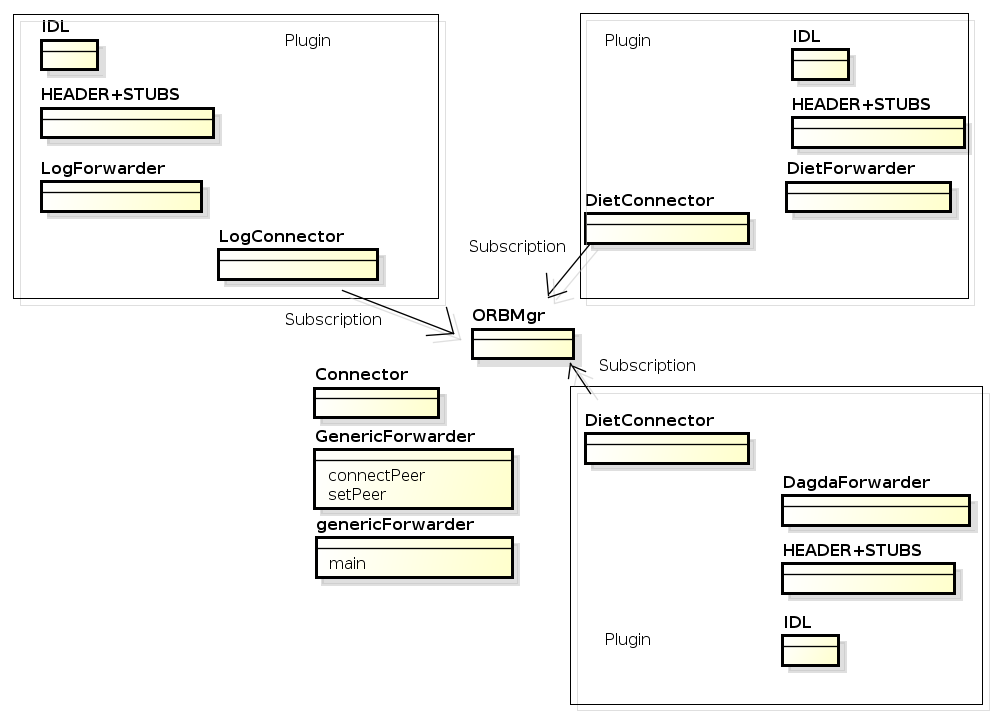
\includegraphics[scale=0.7,angle=90]{fig/component}
\caption{Diagram showing the various component that will be used}
\label{component}
\end{figure}

\subsection*{The class diagram}
\begin{figure}[h!]
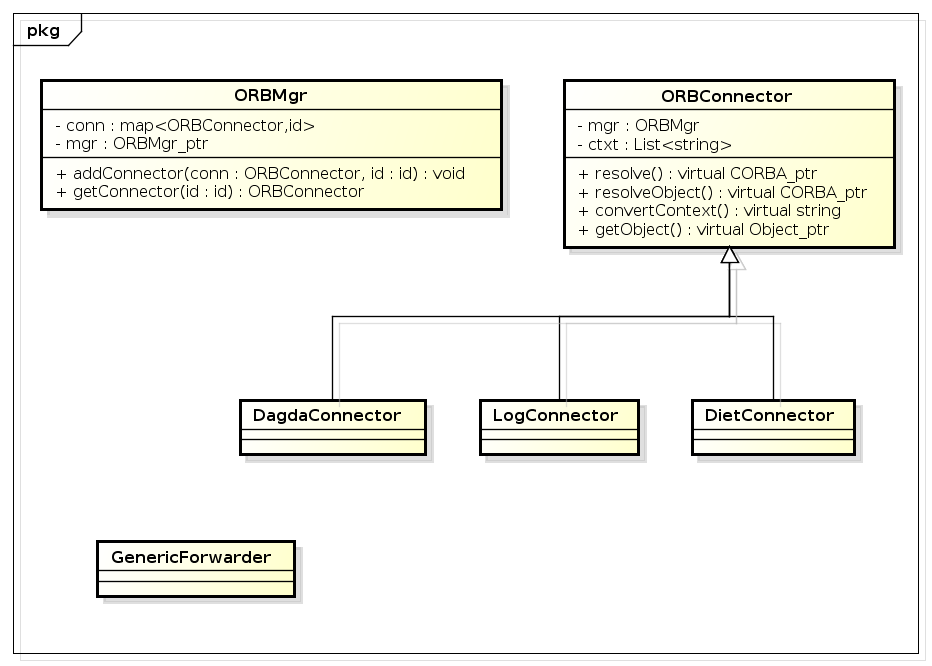
\includegraphics[scale=0.65,angle=90]{fig/class}
\caption{Diagram showing the various classes that will be added}
\label{class}
\end{figure}

\subsection*{The deployment diagram}
\begin{figure}[h!]
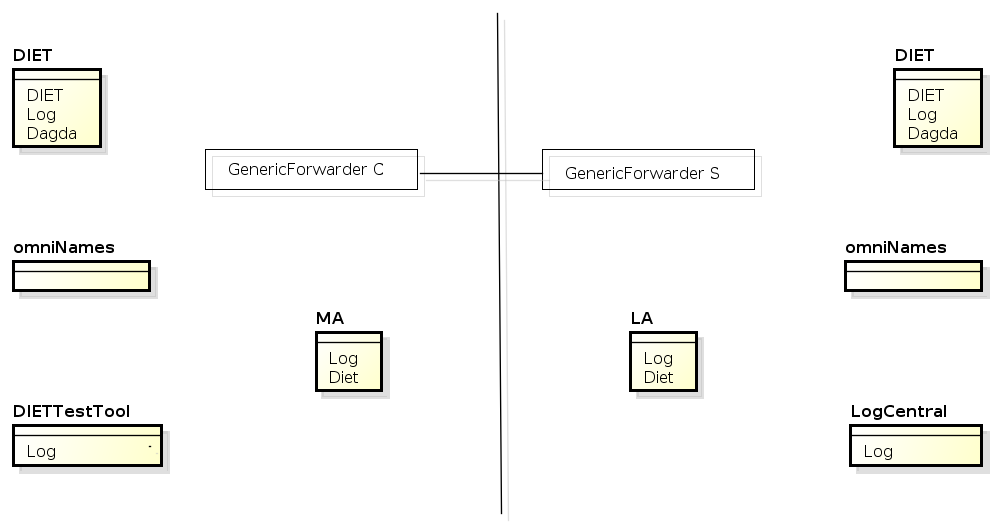
\includegraphics[scale=0.65, angle=90]{fig/deploiement}
\caption{Diagram showing an example of deployment}
\label{deployment}
\end{figure}

\subsection*{The sequence diagram for resolve}
\begin{figure}[h!]
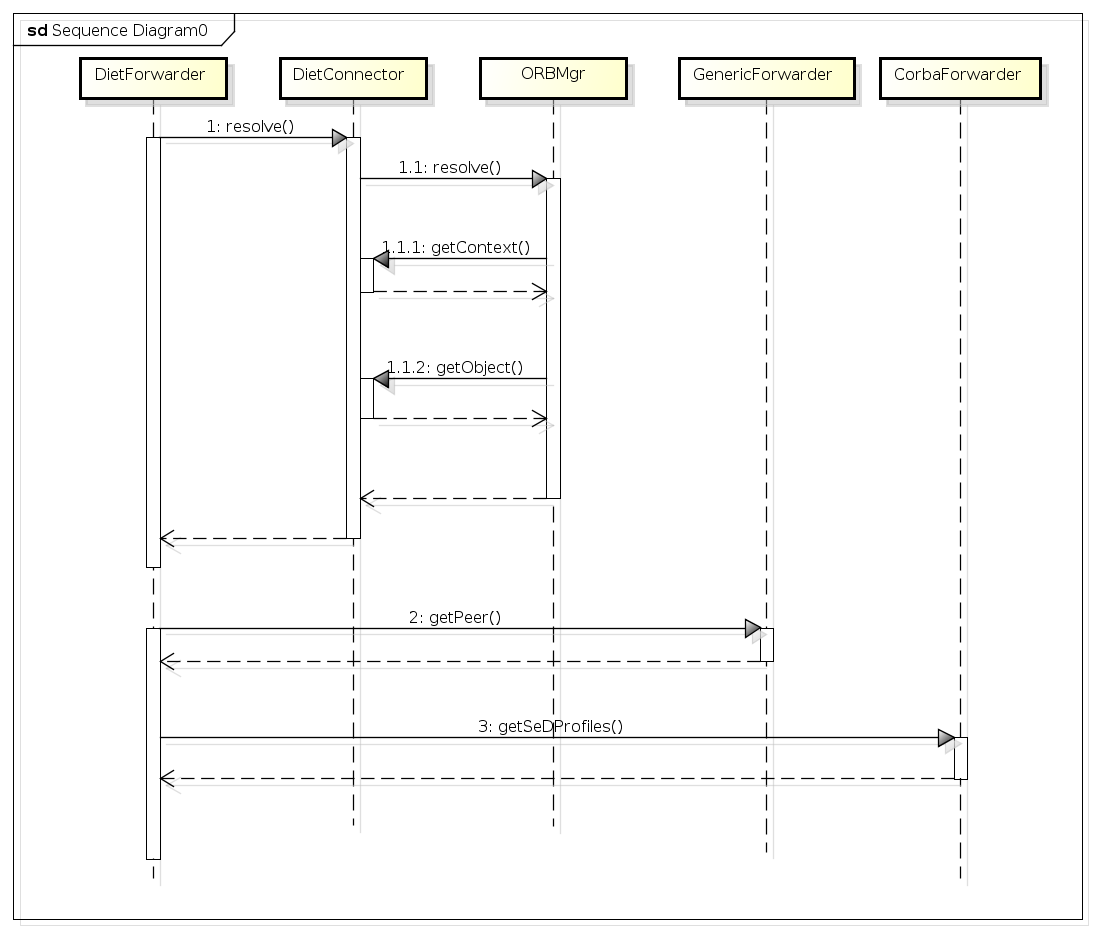
\includegraphics[scale=0.55, angle=90]{fig/sequence}
\caption{Diagram showing the sequence diagram on the resolve function}
\label{sequence}
\end{figure}

\chapter*{Other possibilities}
\section*{The CORBA interceptor}
Haikel presented an idea based on CORBA interceptor. \\
The CORBA norm defines the possibility that the users can make interceptor in some specific points. 
The idea would be to use interceptors to route to the right component that possesses the method required by the object.

\section*{Share the ORBMgr, not the tunnels}
Similar to the presented idea, but the forwarder with the main function are kept separated.

\end{document}
